\section{Proof of the Conditional Initialization Value}
Fix the target-invariant probe $Y$ and the deterministic continuing-program catalogue in main Theorem~\ref{thm:conditional-value}.
Under regime $j$, Gaussian conditioning gives
\begin{align*}
\E_{j,e}[Z_a^2\mid Y=y]&=J_{j,a}^{r}+d_a^2(e^2-r^2)\\
&\quad+2ed_ak_am_j(y)\\
&\quad+k_a^2[m_j(y)^2-s_j^2].
\end{align*}
The observation law and regime posterior do not depend on the unknown fixed $e$.
For any randomized selector, average its risks at $e=r$ and $e=-r$.
The odd cross terms cancel, so the maximum risk is at least $\E_g\min_aL_a(Y)$.
The finitely many scores $L_a$ are even and measurable, and a fixed first minimizer $u$ is even.
Its cross term integrates to zero under each centered Gaussian regime.
Its risk is a nondecreasing affine function of $e^2$ with nonnegative coefficient, and hence its maximum is attained at the endpoints.
It attains the lower bound, proving main Eq.~\eqref{eq:conditional-minimax-value}.
This argument uses classical conditional-loss optimization and symmetry, with the continuing learner and initialization-information class stated explicitly.
The corresponding joint inference principles appear in \maincite{moustakides2012joint}, \maincite{vasconcelos2020observation}, \maincite{reinhard2026minimax} and \maincite{reinhard2024asymptotic}.

The remaining proofs separate state-selection value, invariant observability, the cost of paid inference and the fixed-program comparison.
The error-contrast identity is classical \maincite{harville1974contrasts}; the vector reduction uses the minimax theorem of \maincite{sion1958minimax}.
% Mechanism derivation made before inspecting the new scientific outcomes.
\section{A Finite-Budget Ceiling on State-Selection Value}
An optimal conditional-risk rule does not by itself imply a practically large improvement.
In the scalar Gaussian continuation model one can bound the entire value of using the current noise state, before collecting scientific trajectories.

Fix the same paid probe, remaining budgets, public regime prior and finite catalogue for both rules.
Let $J_{j,a}^{r}$ be the unconditional commitment risk at initialization radius $r$ and let $s_j^2=\operatorname{Var}_j(m_j(Y))$.
Allow a separate common-state transfer coefficient $k_{j,a}$ under each covariance model, including different persistence parameters.
The even conditional risk score is
\begin{align*}
L_a(y)&=F_a(y)+\sum_jp_j(y)k_{j,a}^2S_j(y),\\
F_a(y)&=\sum_jp_j(y)J_{j,a}^{r},\\
S_j(y)&=m_j(y)^2-s_j^2.
\end{align*}
Let $c(y)$ minimize $F_a(y)$ and let $u(y)$ minimize $L_a(y)$, using fixed measurable tie rules.
Both are even selectors and therefore have the initialization-minimax interpretation already proved.
In this section $R(v)$ means the maximum prior-weighted risk over the public scalar initialization interval; evenness attains that maximum at $e=\pm r$.
Put $\mathcal R_j=\max_a k_{j,a}^2-\min_a k_{j,a}^2$.
\begin{equation}
0\le R(c)-R(u)\le4\varphi(1)\sum_j\pi_j\mathcal R_js_j^2.
\label{eq:state-value-ceiling}
\end{equation}
The result is a finite-model upper bound on state information beyond the model posterior; it does not bound the value of identifying the covariance regime itself.
It remains valid for an observable mean-invariant Gaussian probe, using that probe's own explained variances.

For the proof, pointwise optimality gives
\begin{align*}
0\le L_c-L_u&\le\sum_jp_j(k_{j,c}^2-k_{j,u}^2)S_j\\
&\le\sum_jp_j\mathcal R_j|S_j|.
\end{align*}
The first inequality uses $L_u\le L_c$, and the second uses $F_c\le F_u$.
Since $p_j(y)g(y)=\pi_jf_j(y)$,
\[
\mathbb E_g[p_j(Y)|S_j(Y)|]=\pi_j\mathbb E_j|m_j(Y)^2-s_j^2|
=4\varphi(1)\pi_js_j^2.
\]
The last equality follows from the centered Gaussian identity $\mathbb E|G^2-1|=4\varphi(1)$; it also holds at $s_j=0$ by continuity.
Integrating proves Eq.~\eqref{eq:state-value-ceiling}.
The stop action has $k=0$ and fits the same bound.

For a running mean with $N$ applied observations and model-specific sample persistence $\rho=\lambda_j^b$, $|\rho|<1$,
\[
|k_{j,a}|=\frac{|\rho(1-\rho^N)|}{(N+1)|1-\rho|}
\le\frac{|\rho|}{(N+1)(1-|\rho|)}.
\]
For an averaged stable affine-delay learner, assume its impulse response is absolutely summable with sum of absolute values at most $G_*$.
The exact averaging weights obey $|w_t|\le\eta G_*/N$, giving
\[
|k_{j,a}|\le\frac{\eta G_*|\rho|}{N(1-|\rho|)}.
\]
Absolute summability is required here; it is not inferred merely from a numerical finite-horizon check.
For the registered affine steps it follows from the constant-delay characteristic polynomial $z^{D+1}-z^D+\alpha$, with $\alpha=\eta\mu=0.1/(D+1)$.
All roots are inside the unit disk for $0<\alpha<2\sin[\pi/(4D+2)]$.
Indeed for positive small $\alpha$ the root initially at one moves inside while the other roots remain near zero.
At a unit-circle crossing $z=e^{i\omega}$ the equation $z^D(z-1)=-\alpha$ gives a smallest positive crossing magnitude $2\sin[\pi/(4D+2)]$; root continuity excludes an earlier exit.
The registered $\alpha$ is strictly below that magnitude, since $2\sin[\pi/(4D+2)]\ge2/(2D+1)>0.1/(D+1)$.
The impulse generating function $[1-x+\alpha x^{D+1}]^{-1}$ is therefore analytic on a disk of radius greater than one, proving absolute summability.
The finite registered delay set has a finite uniform $G_*$.
If non-stop catalogue horizons are at least a positive constant times the budget scale $B$, and persistence and impulse bounds are uniform over that catalogue, the state-selection value is $O(B^{-2})$.
Relative to a best fixed risk of order $B^{-1}$ this contribution is at most $O(B^{-1})$.
For these stable averaged learners, with finite participation, nonzero private variance, persistence bounded below one and affordable horizons proportional to $B$, that fixed-risk order follows directly: $\sum_tw_t$ tends to a nonzero constant, Cauchy--Schwarz gives a private-variance lower bound proportional to $N^{-1}$, and the weight bound and summable temporal covariance give the matching upper bound.
Covariance-regime adaptation can change the leading $B^{-1}$ variance coefficient, so these two information roles must not be conflated.
The ceiling predicts small state-driven policy differences at long horizons while leaving covariance-regime adaptation as a potential leading-order effect.
\subsection{The second-order state ceiling is attained}
The order $B^{-2}$ can be attained by resource programs of the same running-mean learner.
Take a single Gaussian regime with $\theta=1/3$, $\lambda=1/5$, $Q=8$, $h=8$, $D=0$ and $r^2=49/50$.
A two-observation all-actor probe uses $32$ messages and two clock units.
With total budgets $(80B+32,32B+2)$, its two continuing programs $(q,b)=(2,1)$ and $(8,1)$ have applied horizons $8B$ and $5B$.
Both have leading risk $1/(8B)$.
The invariant contrast is one dimensional, with explained terminal-state variance
\[
s^2=\frac{[\theta(1-\lambda)]^2}{2[\theta(1-\lambda)+1/8]}=\frac{64}{705}.
\]
Let $c$ select the smaller unconditional commitment risk and $u$ the even conditional-risk minimum over these two programs.
For all sufficiently large integer $B$, $c$ selects $(2,1)$.
The exact geometric risk formula yields
\[
B^2(J_{8,1}^{r}-J_{2,1}^{r})\longrightarrow a=\frac{19}{320000},
\]
whereas $B^2(k_{8,1}^2-k_{2,1}^2)s^2\longrightarrow b=13/94000$.
Here $J_{q,b}^{r}$ and $k_{q,b}$ name commitment risk and state transfer, not a new model index.
Since $0<a<b$, the conditional scores cross on a set of positive Gaussian probability.
Writing $G\sim\mathcal N(0,1)$, pointwise minimization and dominated convergence give
\[
\lim_{B\to\infty}B^2[R(c)-R(u)]
=b\,\mathbb E\left[\left(\frac{1187}{2080}-G^2\right)_+\right]>0.
\]
For domination, the scaled risk gaps and state coefficients are bounded by the geometric expansions, so the positive part is bounded by a constant times $1+G^2$.
Thus the state-value ceiling has the sharp budget order in this program class, even with no unknown regime to identify.
The construction establishes strict second-order value, not a first-order gain or confirmation of the separate empirical state-selection test.


% Prospective mechanism analysis, not a new generic value-of-information theorem.
\section{Separating Identification Value, State Value, and the Paid Horizon}
The exact initialization-minimax envelope can be compared with the complete
full-budget fixed catalogue without confusing nominal regime value and actual risk.
For one fixed probe, let $I_{\rm full}$ be the best full-budget fixed risk,
$I_{\rm post}=\min_a\sum_j\pi_jJ_{j,a}^{r}$ the best observation-independent
program after paying the probe, $R_{\rm nom}=\mathbb E_g\min_aF_a(Y)$,
and $R_{\rm rob}=\mathbb E_g\min_aL_a(Y)$.
Let $c(Y)$ minimize $F_a(Y)$ and $u(Y)$ minimize $L_a(Y)$, with fixed even tie
rules. The actual risk of $c$ is $R_c=\mathbb E_gL_{c(Y)}(Y)$, which need not
equal $R_{\rm nom}$.
All post-probe quantities use exactly the same remaining budgets and catalogue,
including stop.
Define
\begin{align*}
C&=I_{\rm post}-I_{\rm full},\\
V_{\rm reg}&=I_{\rm post}-R_{\rm nom},\\
V_{\rm state}&=R_c-R_{\rm rob},\\
T&=\mathbb E_g\sum_jp_j(Y)k_{j,c(Y)}^2S_j(Y).
\end{align*}
Then
\begin{equation}
I_{\rm full}-R_{\rm rob}=V_{\rm reg}+V_{\rm state}-C-T.
\label{eq:research-value-decomposition}
\end{equation}
Here $V_{\rm reg},V_{\rm state}\ge0$ by pointwise minimization.
The signed term $T$ is essential: regime-posterior decisions and continuing
state risk use the same probe. Treating the nominal posterior score as actual
risk would omit precisely the dependence at issue.
The quantity $C$ is the exact, possibly signed, change in the best
fixed risk caused by the paid remaining horizon; no monotonicity of the affine
learner in its horizon is assumed.
This decomposition is an accounting identity using classical decision value,
not a new general information-value theorem.

Let $K$ be the finite state-value ceiling proved above, and define the
post-probe perfect-regime fixed risk
$I_{\rm oracle}=\sum_j\pi_j\min_aJ_{j,a}^{r}$.
Because a posterior-weighted average is at least the posterior average of the
individual regime minima, $R_{\rm nom}\ge I_{\rm oracle}$.
For each $j$, $\mathbb E_g[p_jS_j]=0$.
Centering $k_{j,c}^2$ at the midpoint of its model-specific catalogue range and summing gives $|T|\le K/2$.
Pointwise $\min_aL_a\ge\min_aF_a+\sum_jp_j\min_a(k_{j,a}^2S_j)$.
The expectation of the latter sum is
$-\tfrac12\sum_j(\max_a k_{j,a}^2-\min_a k_{j,a}^2)\mathbb E_g[p_j|S_j|]\ge-K/2$.
Consequently
\begin{align*}
0&\le V_{\rm state}\le K,\\
0&\le V_{\rm reg}\le I_{\rm post}-I_{\rm oracle},\\
|T|&\le K/2,\\
I_{\rm full}-R_{\rm rob}&\le I_{\rm full}-I_{\rm oracle}+K/2.
\end{align*}
Thus $I_{\rm oracle}-K/2\ge I_{\rm full}$ rules out any strict improvement by
any randomized measurable selector following this fixed probe, even if its
regime inference is optimal.
For a desired relative gain $\epsilon>0$, the stronger necessary condition is
$I_{\rm full}-I_{\rm oracle}+K/2\ge\epsilon I_{\rm full}$.
Conversely $V_{\rm reg}>C+K/2$ suffices for a strict paid improvement, since the
state-value contribution is nonnegative and $T\le K/2$.
Neither condition ranges over different probes, estimators, step schedules or
unknown covariance models.
These pre-data criteria explain both when identification can matter and when
more validation seeds cannot rescue a structurally uneconomic probe.

% Research derivation, before inspecting the conditional2h scientific outcomes.
\section{Observable Calibration with an Unknown Target}
The centered-noise pilot assumption can be replaced by an observable invariant statistic in a Gaussian location model.
The projection and generalized least-squares identities below are classical linear-model tools; the issue is whether their statistic supplies the continuing learner's posterior state without revealing the unknown target.

\subsection{Eliminating the target without an oracle}
Let the paid probe be $Z=X\vartheta+W_j$, where the unknown target $\vartheta$ is fixed, the public matrix $X\in\mathbb R^{n\times p}$ has full column rank and $n>p$, and $W_j\sim\mathcal N(0,\Sigma_j)$ under a public finite collection of covariance models.
Choose a deterministic full-row-rank $D\in\mathbb R^{(n-p)\times n}$ satisfying $DX=0$.
Then $Y=DZ=DW_j$ is observable and its law is independent of $\vartheta$.
Its covariance $K_j=D\Sigma_jD^\top$ is positive definite.
If the continuing common state $C$ has cross-covariance $B_j=\operatorname{Cov}_j(C,W_j)$ and variance $T_j$, Gaussian conditioning gives
\begin{align*}
\mathbb E_j[C\mid DZ]&=B_jD^\top K_j^{-1}DZ,\\
\operatorname{Var}_j(C\mid DZ)&=T_j-B_jD^\top K_j^{-1}DB_j^\top.
\end{align*}
The mean-invariant risk selector therefore has the previous conditional-loss and initialization-minimax guarantees when its input is $DZ$ and its model posterior uses $K_j$.
No subtraction of the true target and no improper target prior are needed.
The guarantee is scoped to selectors using this invariant statistic and the specified frozen continuing-program catalogue; it is not optimality over estimators using every part of the raw probe.

\subsection{Projection and determinant identities}
Define
\[
\Pi_j=\Sigma_j^{-1}-\Sigma_j^{-1}X
(X^\top\Sigma_j^{-1}X)^{-1}X^\top\Sigma_j^{-1}.
\]
Then $\Pi_j=D^\top(D\Sigma_jD^\top)^{-1}D$ and
\[
\det(D\Sigma_jD^\top)=
\det\Sigma_j\det(X^\top\Sigma_j^{-1}X)
\frac{\det(DD^\top)}{\det(X^\top X)}.
\]
For the first identity, whiten $\Sigma_j$; both sides become the orthogonal projection onto the complement of the column space of $\Sigma_j^{-1/2}X$, conjugated by $\Sigma_j^{-1/2}$.
For the determinant identity, take orthonormal bases for the columns of $X$ and the rows of $D$.
In that orthogonal basis let $C$ be the covariance block on the contrast coordinates.
The block inverse and determinant formulas give $\det C=\det\Sigma_j\det(U_X^\top\Sigma_j^{-1}U_X)$, where $U_X=X(X^\top X)^{-1/2}$.
Restoring the contrast basis multiplies by $\det(DD^\top)$ and gives the stated formula.
Thus $Z^\top\Pi_jZ$, $B_j\Pi_jZ$ and $B_j\Pi_jB_j^\top$ are exactly target invariant.

For a scalar unknown level, $X=\boldsymbol1$ and $D$ can be the first-difference matrix.
Its two Gram determinants both equal $n$, so the ratio cancels.
Writing $S_j=\boldsymbol1^\top\Sigma_j^{-1}\boldsymbol1$, one obtains
\[
\log\det K_j=\log\det\Sigma_j+\log S_j.
\]
This reduces an $(n-1)$-dimensional determinant to the ordinary innovations determinant and a scalar generalized least-squares information.

\subsection{Linear-time scalar Markov implementation}
For the scalar common-state Markov model with known $\lambda$, noise variance $\theta_j$ and private observation variance $1/Q$, run the usual innovations filter twice with the same deterministic variance sequence: once on the raw probe and once on the all-one vector.
Let their whitened innovations be $u_t$ and $v_t$, with innovation variance $F_t$, and let the two final filtered common-state means be $m_Z$ and $m_1$.
Accumulate
\[
S=\sum_tv_t^2/F_t,\quad T=\sum_tu_tv_t/F_t,\quad U=\sum_tu_t^2/F_t.
\]
Then the invariant quadratic form is $U-T^2/S$, the invariant common-state mean is $m_Z-m_1T/S$, and its explained variance is $\theta_j-P_j-m_1^2/S$.
The formulas follow by substituting the innovations factorization into $\Pi_j$ and using the filtered-state identity $\operatorname{Cov}(C,Z)\Sigma_j^{-1}Z=m_Z$.
Centering the raw probe by its first entry before the calculations leaves $DZ$ unchanged and can reduce cancellation for large unknown target levels.
For the first-difference coordinates, the exact log density is
\[
-\tfrac12\{(n-1)\log(2\pi)+\log\det\Sigma_j+\log S+U-T^2/S\}.
\]
The posterior-state and likelihood calculations require linear time and constant filter-state storage per covariance hypothesis.
All probe observations still incur their message and environment costs, even though the level component is discarded by the selector.

The exact Gaussian affinity for two invariant probe laws is
\[
\rho_D=\frac{\det K_0^{1/4}\det K_1^{1/4}}
{\det[(K_0+K_1)/2]^{1/2}}.
\]
For $\Sigma_j=\theta_jR_\lambda+I/Q$, the covariance midpoint has the same form, so three variance/ones-filter recursions evaluate this affinity.
A zero-threshold likelihood rule has each directional error probability at most $\rho_D$, by applying Markov's inequality to the square root likelihood ratio under each law.
The old full-noise probe's affinity cannot be reused as if projecting out the target were free information.

\subsection{A finite bound on the information cost of removing the target}
Suppose $a_jI\preceq\Sigma_j\preceq b_jI$ uniformly in the probe length, with $a_j>0$, and let $b_{\rm mid}$ bound the covariance midpoint from above.
Write $\rho$ for the full centered-noise affinity and $\rho_D$ for the contrast affinity.
Then
\begin{equation}
1\le\frac{\rho_D}{\rho}
\le C_p:=\frac{b_{\rm mid}^{p/2}}{(a_0a_1)^{p/4}}.
\label{eq:invariant-affinity-cost}
\end{equation}
For the lower bound, complete the contrast coordinates to an invertible linear transformation and apply Cauchy--Schwarz along each discarded coordinate fiber; marginalizing those coordinates increases Gaussian affinity.
For the upper bound, set $U=X(X^\top X)^{-1/2}$.
The determinant identity gives
\[
\frac{\rho_D}{\rho}=
\frac{\det(U^\top\Sigma_0^{-1}U)^{1/4}
\det(U^\top\Sigma_1^{-1}U)^{1/4}}
{\det(U^\top\Sigma_{\rm mid}^{-1}U)^{1/2}}.
\]
The eigenvalues of $U^\top\Sigma_j^{-1}U$ lie between $1/b_j$ and $1/a_j$; substitution proves Eq.~\eqref{eq:invariant-affinity-cost}.
For a fixed nuisance dimension $p$, the bound is independent of the probe length.
Therefore removing an unknown target preserves any existing exponential affinity rate: if $\rho(n)\le Ke^{-In}$, then $\rho_D(n)\le C_pKe^{-In}$.
The sufficient length calculated from this exponential bound incurs an additive term of order $\log C_p/I$, subject also to $n>p$ and full column rank.
This statement does not bound the difference between the two exact minimal confidence-probe lengths without further finite-length control.
This is a determinant/spectral consequence of classical Gaussian error contrasts, not a new general invariance or data-processing principle.

For the registered scalar Markov covariance $\Sigma_j=\theta_jR_\lambda+I/Q$, valid uniform choices are
\[
a_j=Q^{-1}+\theta_j\frac{1-\lambda}{1+\lambda},\quad
b_j=Q^{-1}+\theta_j\frac{1+\lambda}{1-\lambda}.
\]
They follow by bounding the quadratic form of the stationary AR(1) covariance using its spectral density.
The constant can grow with nuisance dimension or near-unit persistence; it does not justify cost-free calibration in those regimes.
The information-rate bound also does not preserve the explained common-state variance, which must be recomputed from $B_j\Pi_jB_j^\top$.

\subsection{Why more data are not automatically justified}
At the same probe schedule, costs and continuation catalogue, observing the full centered noise $W$ is more informative than observing $DW$.
Any invariant selector can be implemented from $W$ by computing $DW$.
Consequently the best full-noise initialization-minimax risk is no larger than the best invariant risk.
This follows from inclusion of policy classes and does not require a new empirical experiment or an unrestricted estimation claim.
The centered-pilot and unknown-target invariant protocols therefore evaluate distinct information classes.
If a new probe schedule is chosen, its different remaining horizons must be recomputed; no unproved monotonicity of the affine learner in its horizon is used.

% Leading result derived before conditional2h outcomes; explicit-constant
% extension derived before reading observable1h outcomes. No new trajectories.
\section{First-Order Regime Value Versus Second-Order State Value}
The state-value ceiling does not rule out a substantial benefit from identifying
the covariance regime: that information can change the leading variance
coefficient of a resource program.
The distinction can be made exact against every affordable fixed training
prefix, rather than only against programs that spend the whole budget.

Consider the running mean with a fixed public initial-error radius $r>0$,
finite positive participation and spacing sets, bounded delay $D$, and
$0\le\lambda\le1-\gamma<1$.
Write the message and clock budgets as $\lfloor\beta_m B\rfloor$ and
$\lfloor\beta_e B\rfloor$, where $\beta_m,\beta_e>0$.
For program $a=(q,b)$ define
\begin{align*}
a_a&=\min\{\beta_m/(h+q),\beta_e/b\},\\
v_j(a)&=q^{-1}+\theta_j\frac{1+\lambda^b}{1-\lambda^b},\\
K_j(a)&=v_j(a)/a_a.
\end{align*}
All programs retain the same running-mean rule; a fixed alternative may choose
any deterministic scheduled prefix, including zero updates, within its budgets.
Let
\begin{align*}
K_\pi&=\min_a\sum_j\pi_jK_j(a),\\
a_j^*&\in\arg\min_aK_j(a),\\
\Delta&=K_\pi-\sum_j\pi_jK_j(a_j^*).
\end{align*}
For two regimes and a fixed tie rule put
$A=\sum_j\pi_j[K_j(a_{1-j}^*)-K_j(a_j^*)]$.
This nonnegative quantity bounds the leading cost of a wrong commitment.
The model laws, prior, initialization radius and probe schedule are public;
the realized regime and initial error are not.

\begin{theorem}[Paid separation from every fixed training prefix]
Suppose a deterministic, target-invariant Gaussian probe has length $n$,
each directional likelihood error is at most $0<\delta<1/2$, and the continuing
programs commit to $a_j^*$ on its decision.
If $\Delta>\delta A$, its signed same-stream upper certificate is below the
minimum worst-initialization prior risk of every full-budget fixed program
and every observation-independent randomized mixture for all sufficiently
large $B$.
More precisely the certified advantage is at least
\[
\frac{\Delta-\delta A}{B}
-\frac{C(n+1)}{B^2},
\]
for a finite model/catalogue-dependent $C$, once all post-probe horizons are
positive fractions of $B$.
If instead the regimes share a leading-coefficient minimizing action, then
$\Delta=0$, and no selector from the maximal-affordable-horizon post-probe
catalogue plus stop, following any such probe with $n=O(\log B)$, can
improve on the best fixed prefix by more than $O((n+1)/B^2)$.
\label{thm:research-leading-separation}
\end{theorem}

The positive claim is relative to a fixed learner and a complete resource-and-
prefix class, not to arbitrary estimators or learning-rate sequences.
The negative claim is an order statement for a specified sublinear paid probe;
it is not an impossibility theorem over all sequential sensing policies.

\subsection{Proof and the role of every hypothesis}
For a fixed action and $N$ applied observations, the exact running-mean risk is
\[
R_{j,a}(N)=\frac{r^2+N/q+
\theta_j[N+2\sum_{s=1}^{N-1}(N-s)\lambda^{bs}]}{(N+1)^2}.
\]
The geometric-sum formula gives
$R_{j,a}(N)=v_j(a)/N+O(N^{-2})$, uniformly on the finite catalogue.
It also gives
$R_{j,a}(N+1)-R_{j,a}(N)=-v_j(a)/N^2+O(N^{-3})$
with an exponentially small remainder.
Since $v_j(a)>0$, each action's risk, and each prior average of it, decreases
strictly beyond a fixed horizon.
Every finite early prefix has positive risk, whereas its maximal affordable
prefix has risk tending to zero.
Thus the optimum over all prefixes eventually uses each candidate action's
maximal horizon, and its global optimum is
$I_{\rm full}=K_\pi/B+O(B^{-2})$.
The same endpoint initialization maximizes all scalar fixed risks; randomizing
fixed programs cannot lower their minimum prior risk.

Subtracting a length-$n$ paid probe changes each maximal horizon from
$a_aB+O(1)$ to $a_aB+O(n+1)$, including rounding and bounded withheld updates.
The correct-program prior risk is therefore
$\sum_j\pi_jK_j(a_j^*)/B+O((n+1)/B^2)$.
The directional-error term is at most $\delta A/B+O((n+1)/B^2)$.
The even invariant likelihood decision cancels the unknown initialization's
odd term; the signed continuing-state correction is $O(B^{-2})$, because
$k_a=O(B^{-1})$ and the probe's explained variance is at most $\theta_j$.
The constants in its truncated-normal factors are finite at fixed $\delta$.
Combining these facts with the fixed-prefix expansion proves the lower bound
on the certified advantage.

For the negative claim, a common leading minimizer gives
$K_\pi=\sum_j\pi_j\min_aK_j(a)$.
The post-probe perfect-regime fixed risk consequently has that same leading
coefficient and a remainder $O((n+1)/B^2)$.
The preceding oracle-plus-half-state-ceiling bound applies to every measurable
randomized selector, whose state-value ceiling is $O(B^{-2})$.
Subtracting the fixed-prefix risk proves the stated upper order.
No monotonicity of an averaged affine learner is invoked in this running-mean
theorem.

\subsection{Existence of an observable finite-confidence probe}
For $\Sigma_j(n)=\theta_jR_\lambda(n)+I/Q$, with distinct positive variances,
the eigenvalues of $R_\lambda(n)$ lie in a fixed positive compact interval.
Both covariance matrices are functions of the same $R_\lambda(n)$.
Each eigen-coordinate contributes a Gaussian affinity factor strictly below
one, uniformly on that interval.
Thus the full centered-noise affinity is at most $\kappa^n$ for some
$\kappa<1$.
The contrast determinant bound gives $\rho_D(n)\le C_1\kappa^n$ for the
unknown scalar target.
Any fixed confidence $\delta>0$ therefore has a finite, observable paid probe.
Its actual directional bound is recomputed after projection, not inherited
from the centered-noise experiment.

\subsection{An explicit sufficient budget threshold}
The sufficiently-large-budget statement has computable, albeit conservative, constants.
All action maxima in this subsection range over non-stop resource pairs; the zero-update program is treated separately.
Write $\rho_a=\lambda^{b_a}$ and define
\[
c_{j,a}=r^2+2v_j(a)+\frac{2\theta_j\rho_a}{(1-\rho_a)^2}.
\]
The geometric sum gives the exact identity
\[
R_{j,a}(N)=\frac{r^2+Nv_j(a)-2\theta_j\rho_a(1-\rho_a^N)/(1-\rho_a)^2}{(N+1)^2},
\]
and hence $|R_{j,a}(N)-v_j(a)/N|\le c_{j,a}/N^2$ for every $N\ge1$.
Let $p_m,p_e$ be the probe's full paid message and clock charges, including any fixed startup cost, and put
\[
L_a(p)=D+1+\max\{(1+p_m)/(h+q_a),(1+p_e)/b_a\}.
\]
For the declared FIFO convention, rounding the two budgets and subtracting the $D$ withheld updates gives
$a_aB-L_a(p)\le N_a^{\rm post}\le a_aB$.
Thus $B\ge2L_a(p)/a_a$ implies
\begin{align*}
\left|J_{j,a}^{r}-\frac{K_j(a)}B\right|&\le\frac{C_{j,a}(p)}{B^2},\\
C_{j,a}(p)&=\frac{4c_{j,a}+2v_j(a)L_a(p)}{a_a^2}.
\end{align*}

The all-prefix lower bound can also avoid an unspecified eventual-monotonicity threshold.
For each action use the prior averages $\bar v_a=\sum_j\pi_jv_j(a)$ and $\bar c_a=\sum_j\pi_jc_{j,a}$, and set $n_{0,a}=\lceil2\bar c_a/\bar v_a\rceil$.
For $N\ge n_{0,a}$ the expansion lower bound is at least $\bar v_a/(2N)$.
If $N<N_{\max,a}/4$ this exceeds $\bar v_a/N_{\max,a}$; if $N\ge N_{\max,a}/4$, the expansion instead bounds the remainder by $16\bar c_a/N_{\max,a}^2$.
For $N<n_{0,a}$, including stop, the initialization term is at least $r^2/(n_{0,a}+1)^2$.
Consequently every prefix obeys
\[
\bar R_a(N)\ge\frac{\bar v_a}{N_{\max,a}}-\frac{16\bar c_a}{N_{\max,a}^2}
\]
whenever $N_{\max,a}\ge\bar v_a(n_{0,a}+1)^2/r^2$.
It follows that
\[
I_{\rm full}\ge\frac{K_\pi}B-\frac{C_F}{B^2},\quad
C_F=\max_a\frac{64\bar c_a}{a_a^2},
\]
provided $B\ge B_F$, where
\[
B_F=\max\left\{\frac{K_\pi}{r^2},\max_a\frac{2L_a(0)}{a_a},
\max_a\frac{2\bar v_a(n_{0,a}+1)^2}{a_ar^2}\right\}.
\]
The zero-update program has risk $r^2$ and is covered by the first term.

Let $c_j=a_j^*$, $w_j=a_{1-j}^*$, and $\kappa=\max_a4\rho_a^2/[a_a^2(1-\rho_a)^2]$.
At $B\ge\max_a2L_a(p)/a_a$, each common-state coefficient has $k_a^2\le\kappa/B^2$.
The explained variance is at most $\theta_j$, and the even decision has centered-square selection correction at most $4\varphi(1)\theta_j\kappa/B^2$.
This also bounds the corresponding signed truncated-normal correction from above.
Using the directional error bound $\delta$ and $K_j(w_j)\ge K_j(c_j)$ therefore gives a certified upper risk
\[
U\le\frac{\sum_j\pi_jK_j(c_j)+\delta A}{B}+\frac{C_U}{B^2},
\]
where
\begin{align*}
C_U=\sum_j\pi_j\{&C_{j,c_j}(p)+\delta[C_{j,c_j}(p)+C_{j,w_j}(p)]\\
&+4\varphi(1)\theta_j\kappa\}.
\end{align*}
Thus a completely explicit sufficient threshold is
\[
B\ge\max\{B_F,\max_a2L_a(p)/a_a\},\quad
B>\frac{C_F+C_U}{\Delta-\delta A},
\]
when $\Delta>\delta A$.
All constants use public model, catalogue and paid-probe quantities.
They may be much more conservative than evaluating the exact finite-budget certificate; no small practical threshold or observed improvement is inferred from this construction.
For a length-$n$ probe with bounded per-observation charges, $C_U=O(n+1)$, recovering the order in the theorem.

\subsection{A rational resource witness on the existing public grid}
Take $Q=8$, $h=8$, $\theta_0=1/20$, $\theta_1=2$, $\lambda=1/5$,
balanced prior, $\beta_m=16$, $\beta_e=4$, and the original
$q\in\{1,2,4,8\}$, $b\in\{1,2,4,8\}$ catalogue.
Exact enumeration of its sixteen leading coefficients yields
\begin{align*}
a_0^*&=(8,4),\quad K_0(a_0^*)=1093/6240,\\
a_1^*&=(2,2),\quad K_1(a_1^*)=5/3,
\end{align*}
while the best balanced fixed coefficient is $K_\pi=773/768$ at $(2,2)$.
The wrong-commitment coefficient is $A=407/1280$.
At directional bound $\delta=1/40$, the sufficient leading margin
$\Delta-\delta A$ is strictly positive (approximately $0.07765$).
Its ratio to $K_\pi$ is approximately $7.71$ percent.
This is a model-population, sufficiently-large-budget witness, not a finite-
grid empirical gain or a claimed threshold value.
All finite budget thresholds and admitted finite-grid designs must still be
computed from the actual paid projected probe and exact learner risk.

\section{Known-Model Population Risk of a Frozen Likelihood Commitment}
The registered finite-seed result and the known-model population effect answer different questions.
The latter can be evaluated without new trajectories for the unchanged binary likelihood rule, including its same-stream state dependence and all paid horizons.
The distributional tool is classical: the positive chi-square mixture is recorded in Solomon, Section2, Eq.(2), with the Gaussian quadratic-form Laplace product in Eq.(3) \maincite{solomon1961quadratic}.
The derivation below supplies its continuing-risk interface, not a new distribution theorem.

\subsection{Diagonal likelihood event and state moment}
Let $K_0\prec K_1$ be the two positive definite contrast covariances, with contrast dimension $d=n-1$ and balanced public prior.
Write $K_0=LL^\top$ and diagonalize
\[
L^{-1}K_1L^{-\top}=V\operatorname{diag}(\ell_i)V^\top,\quad \ell_i>1.
\]
Under true model $j$, the coordinates of $V^\top L^{-1}Y$ have independent variances $\ell_i^j$.
With independent standard normal $G_i$, the likelihood rule selects the high model on
\[
H=\left\{\sum_i a_{j,i}G_i^2>c\right\},\quad c=\sum_i\log\ell_i,
\]
where $a_{0,i}=1-\ell_i^{-1}$ and $a_{1,i}=\ell_i-1$.
Both weight vectors are strictly positive; this positivity uses the ordered variance models and is not asserted for arbitrary covariance pairs.
If $m_j(Y)=\sum_i b_{j,i}G_i$, then $s_j^2=\sum_i b_{j,i}^2$.
Let $p_j=\Pr_j(H)$ and $M_j=\E_j[m_j(Y)^2\mathbf1_H]$.
Every cross-coordinate term vanishes by changing the sign of one $G_i$ while leaving $H$ unchanged.
Consequently $M_j=\sum_i b_{j,i}^2\E[G_i^2\mathbf1_H]$.

For the two frozen post-probe programs, write $J_{j,0}^{r},J_{j,1}^{r}$ for the exact paid stationary risks and $k_0,k_1$ for their common-state coefficients.
The exact worst-initialization model risk is
\begin{align}
R_j^{\rm LR}&=J_{j,0}^{r}+(J_{j,1}^{r}-J_{j,0}^{r})p_j\nonumber\\
&\quad+(k_1^2-k_0^2)(M_j-s_j^2p_j).
\label{eq:population-lr-risk}
\end{align}
The odd initialization term integrates to zero because $H$ is even.
All horizons and coefficients in Eq.~\eqref{eq:population-lr-risk} are those remaining after payment; there is no independent learning reset.
The criterion $\sum_j\pi_jR_j^{\rm LR}<I_{\rm full}$ is therefore an exact known-model comparison for this fixed paid two-commitment rule against the complete fixed-prefix benchmark.
It does not optimize over different probes or all measurable selectors.

\subsection{Positive mixture and explicit series remainder}
Suppress $j$, let $\beta=\min_i a_i>0$, $r_i=1-\beta/a_i\in[0,1)$, and define
\begin{align*}
C(z)&=\prod_i(\beta/a_i)^{1/2}(1-r_iz)^{-1/2}\\
&=\sum_{k\ge0}c_kz^k.
\end{align*}
The coefficients are nonnegative and $C(1)=1$.
Logarithmic differentiation gives
\[
c_0=\prod_i(\beta/a_i)^{1/2},\quad
c_k=\frac1k\sum_{l=1}^k\left(\frac12\sum_i r_i^l\right)c_{k-l}.
\]
Substitute $z=(1+2\beta t)^{-1}$ into the Laplace product $\prod_i(1+2a_it)^{-1/2}$.
It becomes a probability mixture of the transforms of $\beta\chi^2_{d+2k}$, proving the classical series.
Define $h_k$ by the nonnegative generating function
\[
\sum_{k\ge0}h_kz^k=C(z)\sum_i\frac{b_i^2\beta/a_i}{1-r_iz}.
\]
Its coefficient mass is $\sum_kh_k=s^2$.
Weighting one Gaussian coordinate by $G_i^2$ increases that coordinate's chi-square degrees of freedom from one to three.
Thus, with $\overline F_v$ the standard chi-square upper-tail function,
\begin{align*}
p&=\sum_{k\ge0}c_k\overline F_{d+2k}(c/\beta),\\
M&=\sum_{k\ge0}h_k\overline F_{d+2+2k}(c/\beta).
\end{align*}
For sums retained through $K$, denote the partial values by $p_K,M_K$ and let
$\epsilon_p=1-\sum_{k\le K}c_k$, $\epsilon_M=s^2-\sum_{k\le K}h_k$.
In exact arithmetic,
\[
p_K\le p\le p_K+\epsilon_p,\quad
M_K\le M\le M_K+\epsilon_M.
\]
The corresponding risk interval width is at most
\begin{align*}
&|\Delta J_j-\Delta k^2s_j^2|\epsilon_p+|\Delta k^2|\epsilon_M,\\
&\Delta J_j=J_{j,1}^{r}-J_{j,0}^{r},\quad \Delta k^2=k_1^2-k_0^2.
\end{align*}
Floating-point rounding and special-function error are separate from this exact series-truncation statement.

\subsection{Outcome-known diagnosis of the unchanged gate}
Deterministic numerical evaluation retains all128 observable-study designs and their original29 admissions and99 fixed fallbacks.
It approximates the population normalized fixed-minus-gate gain by $0.00875334$, below the registered $0.01$ practical threshold, and the uncertified-probe-minus-gate gain by $0.190124$.
The maximum normalized omitted-series-mass risk width at the computed coefficients is below $3.7\times10^{-14}$; this is a truncation diagnostic, not a rigorously rounded interval or a sampling confidence limit.
Scaled chi-square identities and independent two-dimensional quadrature check the probability and selected-state-moment formulas.
Independent characteristic-function integration checks the actual probe laws separately.
This outcome-known calculation neither changes an action nor replaces the registered negative finite-seed decision.
It explains why simply adding seeds is not a principled response to the unmet practical-size target on this grid.

% Matrix extension; no vector empirical superiority is inferred.
\section{A Matrix Form of Paid Calibration Value}
The scalar initialization argument relies on the fact that every program contracts all error directions by the same scalar.
For vector learners this property can fail, so replacing every program's initial error by its separate worst direction can produce an unattainable score.
The following reduction keeps one common unknown initialization across the whole observation space.
Its minimax interchange is a classical convex-game argument; the specific object is the finite-dimensional covariance problem for paid continuing programs.

\subsection{Information, affine continuation and integrability}
Let $e\in\mathbb R^d$ satisfy $e^\top P e\le r^2$, with public $P\succ0$ and $r>0$.
The unobserved $e$ is fixed across the experiment and does not affect the centered calibration-probe law.
Fix a public prior over a finite set of Gaussian noise models $j$.
For each model, the probe law $Y\sim\mathcal N(0,\Sigma_j)$ is nonsingular, the conditional common state $C\in\mathbb R^k$ has linear mean $m_j(y)$ and constant covariance, and the continuing Gaussian noise is jointly specified.
Both the paid probe schedule and every subsequent candidate program are frozen before observing $Y$.
Under model $j$ and program $a$, suppose the terminal error has conditional mean $A_{j,a}e+B_{j,a}m_j(y)$ and conditional covariance $V_{j,a}\succeq0$.
All matrices are known and deterministic, and their horizons include the probe charges, affine delay and withheld updates.
An implementable selector sees $Y$ and these public objects but not $e$ or $j$.
In particular the centered calibration observation must be obtainable without subtracting an unknown target.

Let $g$ be the mixture density and $p_j(y)$ its model posterior, and define
\begin{align*}
H_a(y)&=\sum_jp_j(y)A_{j,a}^\top A_{j,a},\\
Q_a(y)&=\sum_jp_j(y)\{\operatorname{tr}V_{j,a}+\|B_{j,a}m_j(y)\|^2\}.
\end{align*}
Both functions are even in $y$, $H_a$ is bounded, and $Q_a$ is integrable under $g$ because the catalogue is finite and Gaussian second moments are finite.
The posterior squared loss equals $e^\top H_a(y)e+Q_a(y)$ plus a term linear in $e$ and odd in $y$.
Consequently symmetrizing a selector cannot increase its maximum risk over the centrally symmetric error set.

\subsection{Exact covariance reduction}
Let $\Delta_{\rm even}$ be the measurable randomized even selectors over the finite catalogue, and put
\[
\mathcal S=\{S\succeq0:\operatorname{tr}(PS)\le r^2\}.
\]
Then the exact robust risk following the paid probe is
\begin{align}
&\inf_{\delta}\sup_{e^\top Pe\le r^2}R_e(\delta)\nonumber\\
&=\max_{S\in\mathcal S}\int\min_a\{\operatorname{tr}[H_a(y)S]+Q_a(y)\}g(y)\,dy.
\label{eq:matrix-covariance-envelope}
\end{align}
The minimax error-direction problem has therefore reduced to a concave maximization over a finite-dimensional initialization covariance.
The probe integration is still present; its numerical approximation requires its own accuracy justification.

To prove Eq.~\eqref{eq:matrix-covariance-envelope}, first symmetrize any selector, using $R_e(\delta^{\rm sym})=[R_e(\delta)+R_{-e}(\delta)]/2$.
For an even selector define $M_\delta=\mathbb E_g\sum_a\delta_a(Y)H_a(Y)$ and $c_\delta=\mathbb E_g\sum_a\delta_a(Y)Q_a(Y)$.
Its risk is $e^\top M_\delta e+c_\delta$.
The convex hull of $ee^\top$ over $e^\top Pe\le r^2$ is exactly $\mathcal S$: diagonalize $P^{1/2}SP^{1/2}$ and express it as a convex combination of rank-one radius-$r$ errors, with any unused mass at zero.
Hence the worst-case risk equals $\max_{S\in\mathcal S}\operatorname{tr}(M_\delta S)+c_\delta$.

The set $\mathcal S$ is compact and convex.
Regard each component of $\delta$ as an element of $L^\infty(g)$.
The probability-simplex constraints and evenness are weak-star closed, so $\Delta_{\rm even}$ is weak-star compact and convex.
The integrable functions $H_a,Q_a$ make the objective continuous and affine in each argument for the weak-star and finite-dimensional topologies.
The classical minimax interchange applies.
At fixed $S$, an even first minimizer of the finitely many even scores minimizes the integral, proving Eq.~\eqref{eq:matrix-covariance-envelope}.
Continuity and compactness give attainment in the primal and covariance-dual problems.

\subsection{A dual maximizer does not license arbitrary tie breaking}
There exists a saddle pair $(\delta^*,S^*)$; an arbitrary pointwise minimizer at a dual maximizer $S^*$ need not be a minimax selector.
Its tie randomization must also make $S^*$ a worst-case covariance for that selector.
For example take an irrelevant nonsingular centered Gaussian probe, zero continuation noise, $P=I_2$, $r=1$ and two programs with $A_0=\operatorname{diag}(1,0)$ and $A_1=\operatorname{diag}(0,1)$.
The dual objective is $\min(S_{11},S_{22})$, maximized at $S^*=I_2/2$ with value $1/2$.
Both actions tie everywhere at $S^*$.
Selecting the first action deterministically has worst-case risk one; mixing the two actions equally attains $1/2$.
Thus the scalar fixed tie rule cannot be transported to arbitrary matrix contractions without checking the saddle condition.
If the minimizing action is unique $g$-almost everywhere at a dual maximizer, the unique pointwise minimizer is the saddle selector because a primal optimizer exists and must minimize there.

\subsection{The strongest fixed comparison is itself a semidefinite program}
For the full-budget no-probe catalogue let $\overline H_a^{\rm full}$ be the prior average of $A_{j,a}^\top A_{j,a}$ and $\overline Q_a^{\rm full}$ its full-budget zero-initialization risk.
A fixed randomized program uses a probability vector $w\in\mathcal W=\{w\ge0:\sum_aw_a=1\}$ independent of the calibration observations and unknown initialization.
Its optimum worst-case risk $I_{\rm fix}$ is the value of
\begin{equation}
\begin{aligned}
\underset{w\in\mathcal W,\,t\in\mathbb R}{\operatorname{minimize}}\quad
&r^2t+\sum_aw_a\overline Q_a^{\rm full}\\
\text{subject to}\quad&\sum_aw_a\overline H_a^{\rm full}\preceq tP.
\end{aligned}
\label{eq:matrix-fixed-SDP}
\end{equation}
The constraint bounds the largest generalized initialization eigenvalue exactly, so this is a semidefinite program over a finite catalogue.
The example above proves why a comparison restricted to deterministic fixed programs can overstate a matrix selector's benefit.
Strict superiority to every fixed randomized programme in this catalogue is attainable after the specified paid probe if and only if the value in Eq.~\eqref{eq:matrix-covariance-envelope} is strictly less than $I_{\rm fix}$.
The reverse inequality is an impossibility certificate for this probe and catalogue, rather than a statement about every possible adaptive experiment.

With $P=I$ and scalar contractions $A_{j,a}=d_aI$, every unknown direction gives the same coefficient and the maximizing covariance can be taken on the radius boundary.
The formula reduces to the previously proved scalar even conditional-risk selector, and a fixed random mixture cannot improve its linear scalar endpoint objective.
The scalar simulations evaluate this reduction; the matrix characterization is analytical.


\section{Conditional-State Validation and the Paid-Probe Boundary}
The conditional-state study fixes nine policies, two learners, sixteen families, four budget scales, two covariance regimes, both initial-error signs and 64 independent paired master seeds.
Its 294,912 trajectories use a separate known-zero calibration pilot, rather than unknown-target contrasts.
Public control rules see neither the realized regime, true target, initial-error sign nor future observations.
The two evaluation-only oracles are labeled separately.
The post-probe catalogue contains stop and every original participation--spacing program at its maximal affordable horizon; the full-budget fixed benchmark uses the corresponding full-budget catalogue and stop.
The fixed-minus-conditional and posterior-marginal-minus-conditional contrasts are averaged equally over all 128 designs, both regimes and both signs within each master seed, normalized by each design's pre-data population best balanced fixed risk.
The registered positive decision requires two positive one-sided 99.5 percent paired-bootstrap lower bounds and at least one percent mean fixed-policy improvement.
The bootstrap uses 10,000 resamples and approximate percentile coverage.

The registered decision is negative.
The fixed-minus-conditional mean is $-0.993855$, with descriptive 95 percent interval $[-1.015340,-0.973059]$.
The posterior-marginal-minus-conditional mean is $-1.12\times10^{-5}$, with interval $[-1.06\times10^{-4},5.67\times10^{-5}]$.
There are 87 adverse fixed-comparison design means out of 128.
Fixed-minus-conditional means at scales 32, 128, 512 and 2048 are respectively $-3.728961$, $-0.237679$, $-0.052351$ and $0.043571$.
Thus selecting a continuing program after paying a feasible pilot does not replace the economic decision of whether to buy that pilot.
The state-information correction gives no confirmed incremental gain over the posterior-marginal rule on this grid.

\begin{table*}[t]
\centering
\caption{Complete conditional-state study: descriptive equal-cell means over all families, budgets, regimes and initialization signs.}
\label{tab:conditional-all-policies}
\begin{tabular}{lrrrr}
\toprule
Policy & Squared risk & Normalized risk & Messages & Clock units\\
\midrule
Robust conditional &0.098475&2.009532&18509.68&2468.19\\
Known-error oracle (evaluation only)&0.098169&2.009318&18509.47&2466.34\\
Posterior marginal&0.098476&2.009521&18509.70&2468.19\\
Legacy risk gate&0.077053&1.270375&18510.16&2463.49\\
Information only&0.098477&2.009903&18509.93&2467.45\\
All actors&0.113417&2.962129&19040.00&680.00\\
Fixed $(q,b)=(2,1)$&0.061440&1.326310&19037.50&1903.75\\
Best balanced full-budget fixed&0.051784&1.015677&18187.84&2560.36\\
Known-regime fixed (evaluation only)&0.051252&0.987827&18508.48&2509.63\\
\bottomrule
\end{tabular}
\end{table*}

\begin{figure*}[t]
\centering
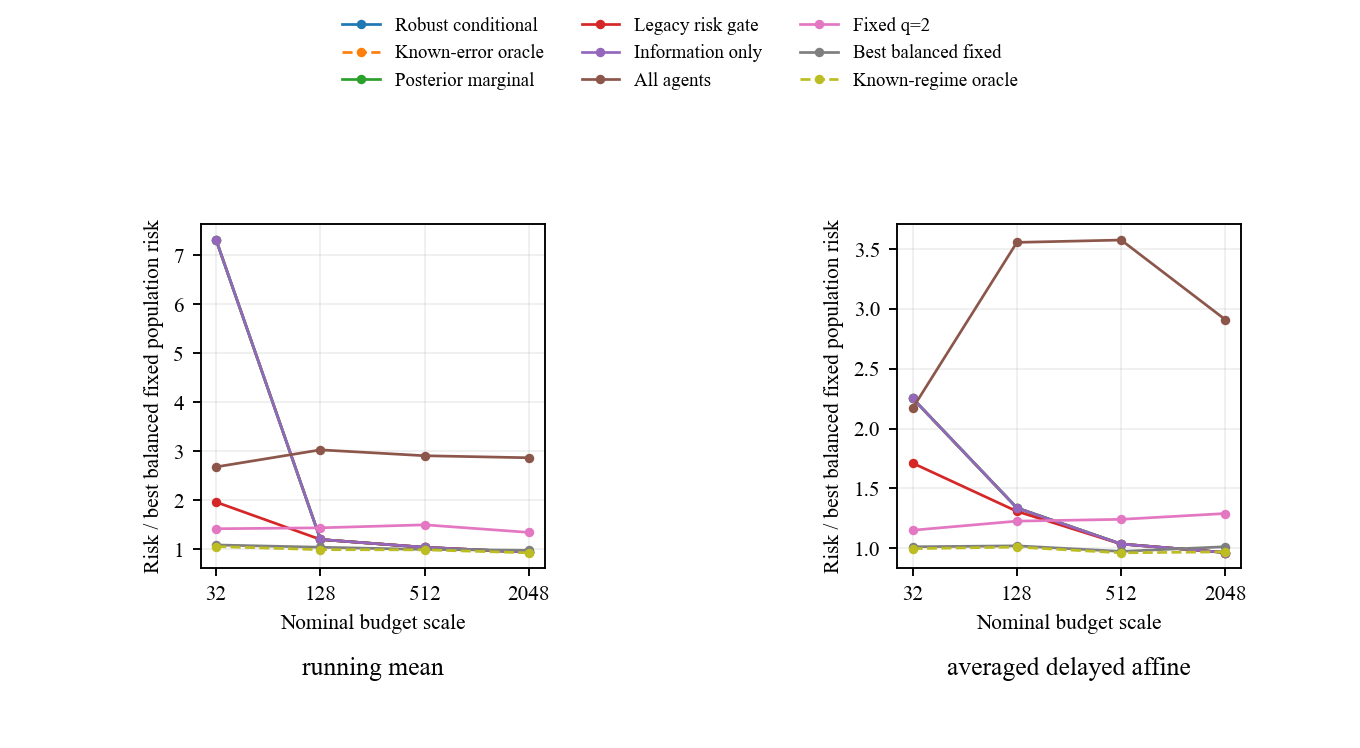
\includegraphics[width=\textwidth]{figures/conditional_budget_20261021.png}
\caption{Conditional-state study, all nine policies: normalized risk against budget scale, separately for the two learners. Coincident curves are not graphically offset.}
\label{fig:conditional-budget}
\end{figure*}
\begin{figure*}[t]
\centering
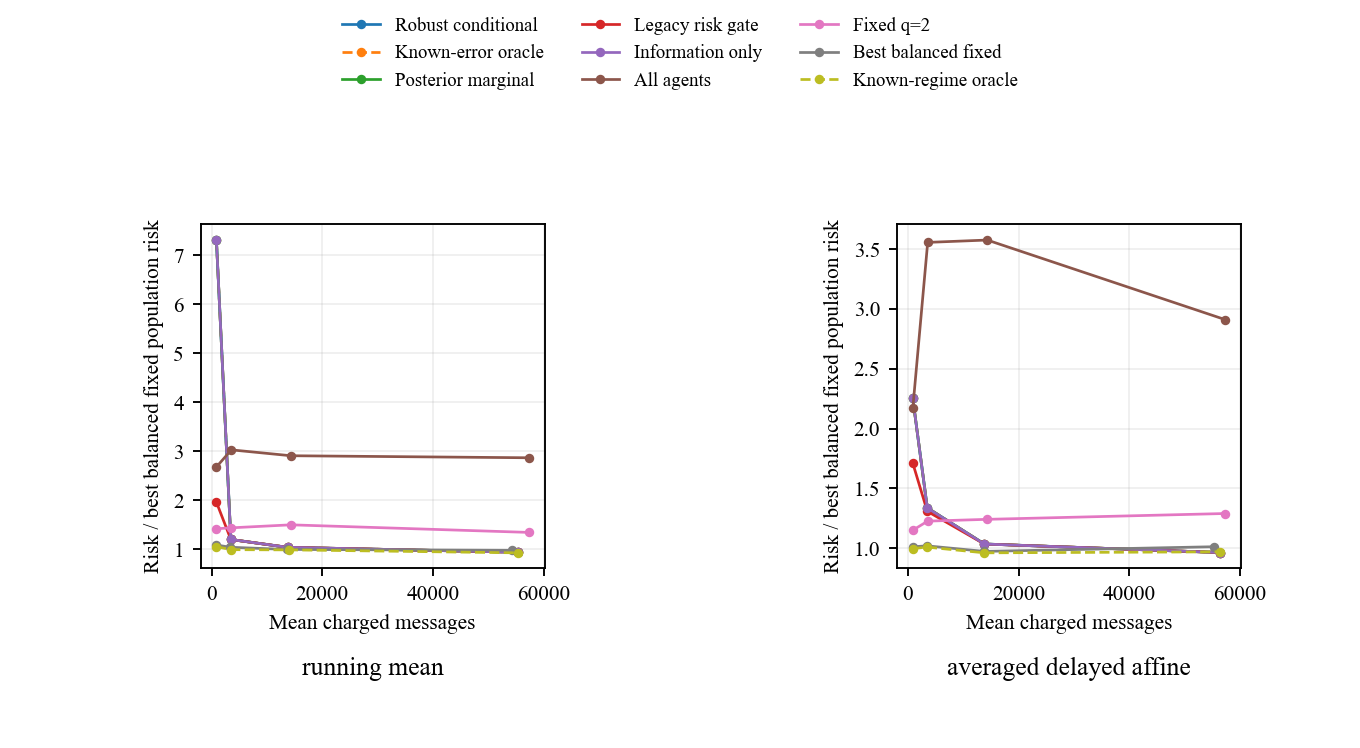
\includegraphics[width=\textwidth]{figures/conditional_messages_20261021.png}
\caption{All conditional-state policies against actual paid messages; points correspond to distinct budget experiments.}
\label{fig:conditional-messages}
\end{figure*}
\begin{figure*}[t]
\centering
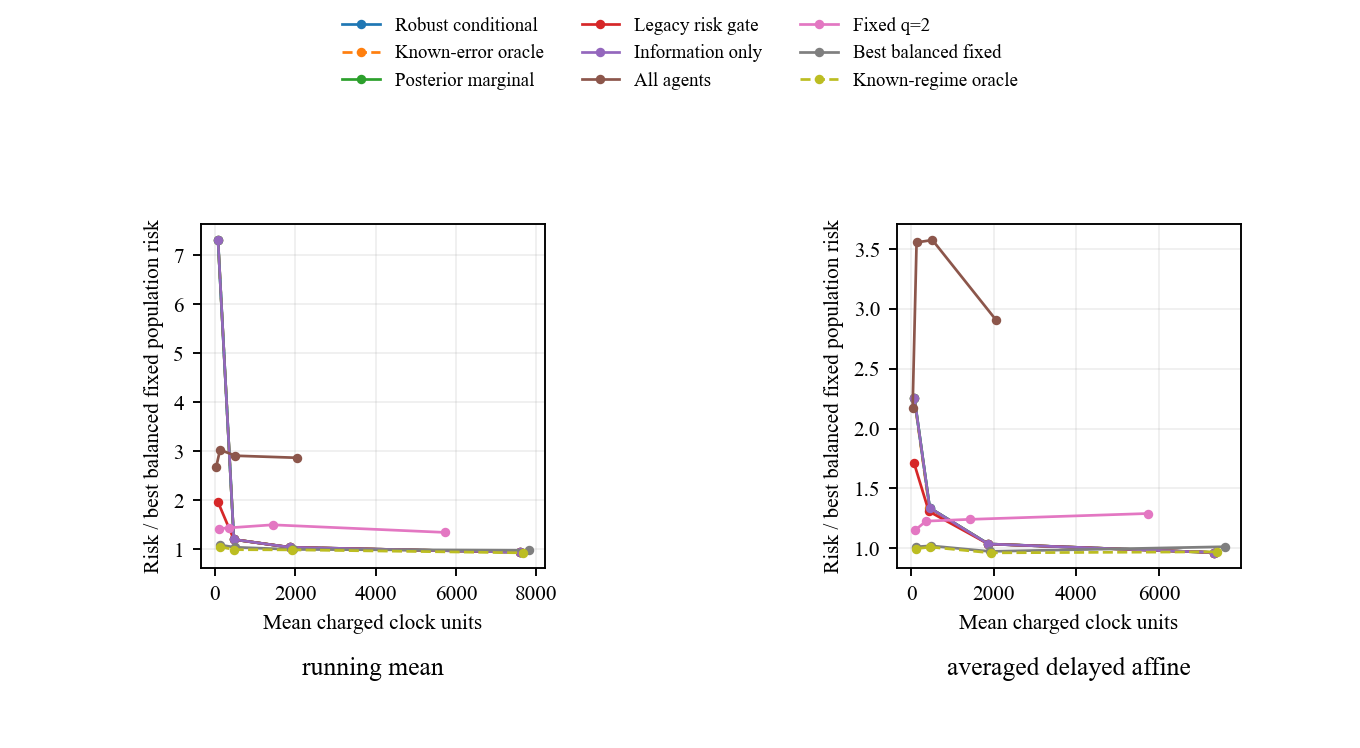
\includegraphics[width=\textwidth]{figures/conditional_clock_20261021.png}
\caption{All conditional-state policies against paid clock units; neither the message nor clock plot asserts equal-cost pointwise dominance.}
\label{fig:conditional-clock}
\end{figure*}
\begin{figure*}[t]
\centering
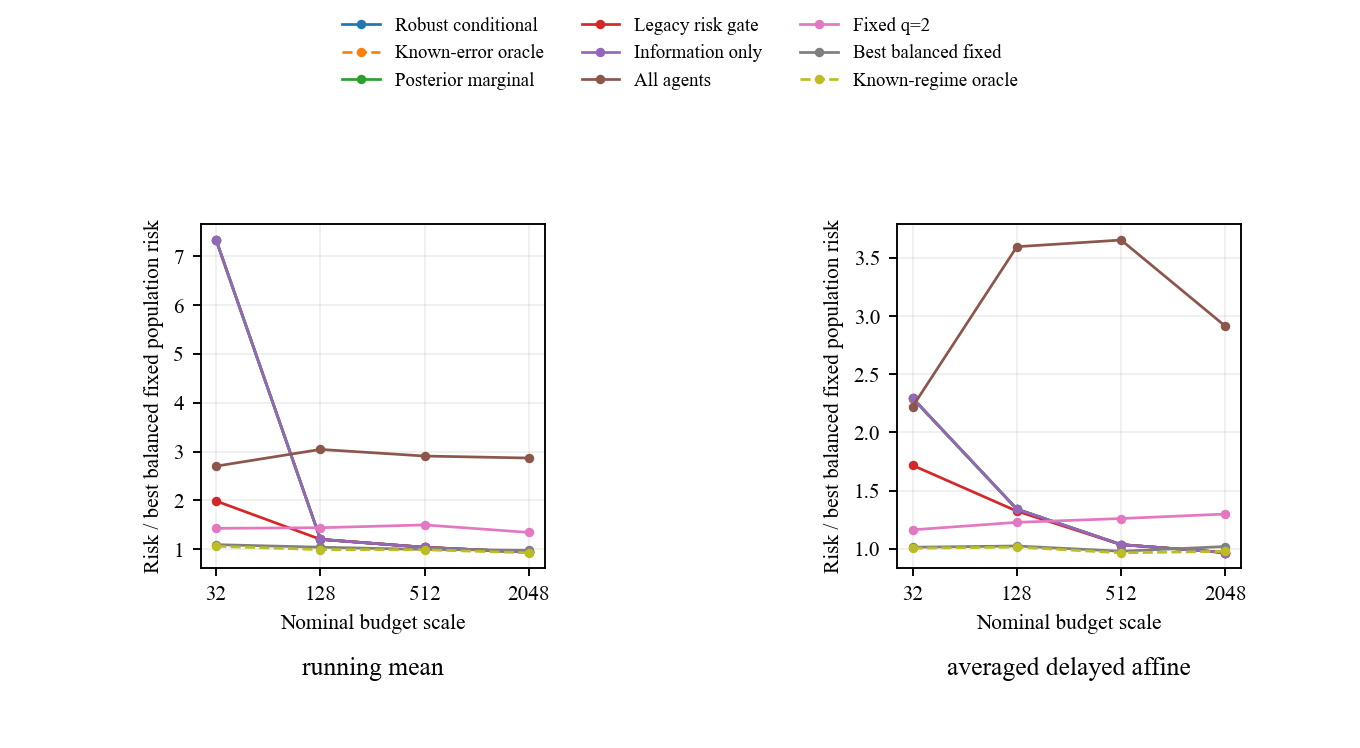
\includegraphics[width=\textwidth]{figures/conditional_learner_budget_20261021.png}
\caption{Conditional-state study using the larger empirical mean over the two fixed initial-error signs in each learner and budget.}
\label{fig:conditional-sign}
\end{figure*}
\section{Observable Paid-Risk Gate Against All Fixed Prefixes}
\subsection{Prospective model, information and baseline}
The observable-probe study was specified before the conditional-state study's outcomes were inspected.
It retains nine policies, two learners, all sixteen families and four budget scales, both true covariance regimes and both hidden initial-error signs.
There are 64 fresh paired master seeds, $20591001,\ldots,20591064$, giving $294912$ policy trajectories and the same number of full semantic replays.
The known binary models, balanced public prior, radius $r=1$, original participation--spacing sets, learner steps and paid FIFO convention are unchanged.
The raw probe is target contaminated: it observes target plus noise for the running mean, and half the target plus noise for the affine learner at initial parameter zero.
The deployment uses only first differences and the equivalent two-filter invariant likelihood, not the unknown target, initial-error sign, true regime or future observations.
Both target signs use the same potential noise stream across policies; the parameter and target are translated together.

The probe uses all $Q$ actors at unit spacing and the smallest length $n\in\{2,\ldots,4096\}$ whose projected Gaussian affinity is at most $0.025$.
The two post-probe commitments minimize the appropriate model's exact risk over stop and every original participation--spacing pair at its maximal affordable remaining horizon.
The signed prior-risk upper bound is compared with the best balanced full-budget fixed risk before collecting any probe observations.
Unlike the preceding study, that fixed benchmark includes every affordable scheduled training prefix for every original pair, plus stop, at the same learner and step.
An independent scalar recurrence checks its population normalizer; evaluation-only known-regime fixed programs receive the same complete prefix catalogue.
No choice of learning-rate sequence or estimator outside the declared class is included.

The certified gate probes only on a strict certificate improvement and otherwise executes that strongest fixed prefix without a probe.
Other policies are an uncertified invariant likelihood commitment whenever probing is feasible, a no-carryover admission ablation, posterior-marginal selection over the full post-probe catalogue, all actors, fixed $(2,1)$, and two privileged evaluation references.
The known-target centered-pilot reference and known-regime fixed reference are not deployable policies or universal risk lower bounds.
All probe and scheduled training observations are paid, including withheld terminal updates.
An infeasible probe uses the strongest fixed backstop.

\subsection{Registered primary decision and every policy}
The paired master-seed estimands normalize each design by its pre-data balanced population best-fixed risk and weight all 128 designs, both regimes and both signs equally.
The two co-primary contrasts are fixed minus certified gate, and uncertified invariant likelihood probe minus certified gate.
The registered positive decision requires both one-sided 99.5 percent bootstrap lower bounds above zero and fixed-minus-gate mean at least $0.01$.
There are 10,000 fixed-seed bootstrap resamples; coverage is approximate percentile coverage, not a finite-sample confidence theorem.

The registered practical-positive decision is not confirmed.
Fixed-minus-gate mean is $0.00444303$, with one-sided lower bound $-0.00317725$ and descriptive 95 percent interval $[-0.00119855,0.00999250]$.
Uncertified-probe-minus-gate mean is $0.170210$, with lower bound $0.148124$ and descriptive interval $[0.153487,0.187211]$.
The former misses both its confidence and practical-size conditions; the latter supports the value of not buying an uneconomic probe.
There are 9/128 adverse fixed-comparison design means and 20/128 adverse uncertified-probe comparison means.
At scales 32, 128, 512 and 2048 the fixed-minus-gate means are respectively $0$, $0$, $0.00989743$ and $0.00787469$.
The running-mean aggregate is $0.00876160$ and the affine aggregate $0.000124462$.
These secondary descriptions do not replace the all-design primary decision.

There are 116 feasible probes, 29 certificate admissions and 99 exact fixed-prefix fallbacks.
All 25,344 nonadmitted policy rows have exactly the paired fixed policy's terminal error and paid costs.
Corrected and no-carryover gates coincide on all 32,768 paired rows; there is again no evidence of incremental empirical decision value for the correction on this grid.
The two endpoint signs check information roles; uniform initialization risk control comes from the analytical envelope, not empirical coverage of every initialization.

\begin{table*}[t]
\centering
\caption{Observable paid-gate study: all nine policies, descriptive equal-cell means over 512 learner--family--budget--regime--sign cells per policy, with 64 seeds per cell.}
\label{tab:observable-all-policies}
\begin{tabular}{lrrrr}
\toprule
Policy & Squared risk & Normalized risk & Messages & Clock units\\
\midrule
Observable certified gate&0.050644&0.972057&18461.16&2516.16\\
Known-target pilot (evaluation only)&0.067765&1.141980&18504.42&2470.74\\
Observable uncertified likelihood&0.067856&1.142267&18506.78&2472.50\\
No-carryover admission&0.050644&0.972057&18461.16&2516.16\\
Observable posterior marginal&0.067856&1.142201&18505.12&2472.96\\
All actors&0.113505&2.941037&19040.00&680.00\\
Fixed $(q,b)=(2,1)$&0.060679&1.346523&19037.50&1903.75\\
Best balanced full-budget fixed prefix&0.050640&0.976501&18187.84&2560.36\\
Known-regime fixed (evaluation only)&0.050115&0.949517&18508.48&2509.63\\
\bottomrule
\end{tabular}
\end{table*}

The nearly equal raw pooled risks do not favor the gate over strongest fixed: $0.0506443$ versus $0.0506405$.
Raw pooled and design-normalized contrasts give different weights to heterogeneous designs, so neither is silently substituted for the registered estimand.
The gate sends more messages but uses slightly fewer clock units than strongest fixed; no equal-realized-cost dominance follows.
The full mechanism diagnosis is therefore bounded: observable risk admission avoids the losses of paying a feasible pilot indiscriminately, but the study does not demonstrate a practically necessary advantage over a well-chosen fixed prefix.
No extra seeds, favorable-subset replacement or outcome-dependent threshold change is used to alter that decision.

